\documentclass{article}
\usepackage{titling}
\usepackage{amsmath}
\usepackage{graphicx}
\usepackage{float}
\usepackage{multirow}
\usepackage{arydshln}

\setlength{\droptitle}{-10em}
\title{AP Statistics Part 1 Practice}
\author{Rishi Salwi and Eric Zheng}

\begin{document}
\maketitle

\begin{enumerate}
  % Question 1
  % I'll organize all the plots once they're done
  \item The following plots were created:
    \begin{enumerate}
      \item Stem and leaf plot:
        \begin{figure}[H]
          \centering
          \caption{Stem and Leaf Plot of Women's Heights (in.)}
          \begin{tabular}{r|cccc}
  \hline
  Stem & \multicolumn{4}{l}{Leaf} \\
  \hline
  50. & 2 &   &   &   \\
  51. &   &   &   &   \\
  52. &   &   &   &   \\
  53. & 2 &   &   &   \\
  54. &   &   &   &   \\
  55. &   &   &   &   \\
  56. & 7 &   &   &   \\
  57. & 4 & 9 &   &   \\
  58. & 6 & 9 &   &   \\
  59. & 0 & 3 & 3 &   \\
  60. &   &   &   &   \\
  61. & 4 &   &   &   \\
  62. & 1 & 1 & 4 & 4 \\
  63. & 1 & 1 & 3 &   \\
  64. &   &   &   &   \\
  65. & 4 & 6 &   &   \\
  66. &   &   &   &   \\
  67. & 7 &   &   &   \\
  68. & 5 & 5 &   &   \\
  69. &   &   &   &   \\
  70. & 4 & 5 &   &   \\
  \hline
\end{tabular}

        \end{figure}
      \item Frequency table:
        \begin{table}[H]
          \centering
          \caption{Frequency Table of Women's Heights (in.)}
          \begin{tabular}{c c}
  \hline
  Interval & Frequency \\
  \hline
  $[50.2, 52.7)$ & 1 \\
  $[52.7, 55.2)$ & 1 \\
  $[55.2, 57.7)$ & 2 \\
  $[57.7, 60.2)$ & 6 \\
  $[60.2, 62.7)$ & 5 \\
  $[62.7, 65.2)$ & 3 \\
  $[65.2, 67.7)$ & 2 \\
  $[67.7, 70.2)$ & 3 \\
  $[70.2, 72.7)$ & 2 \\
  \hline
\end{tabular}

        \end{table}
      \item Histogram:
        \begin{figure}[H]
          \centering
          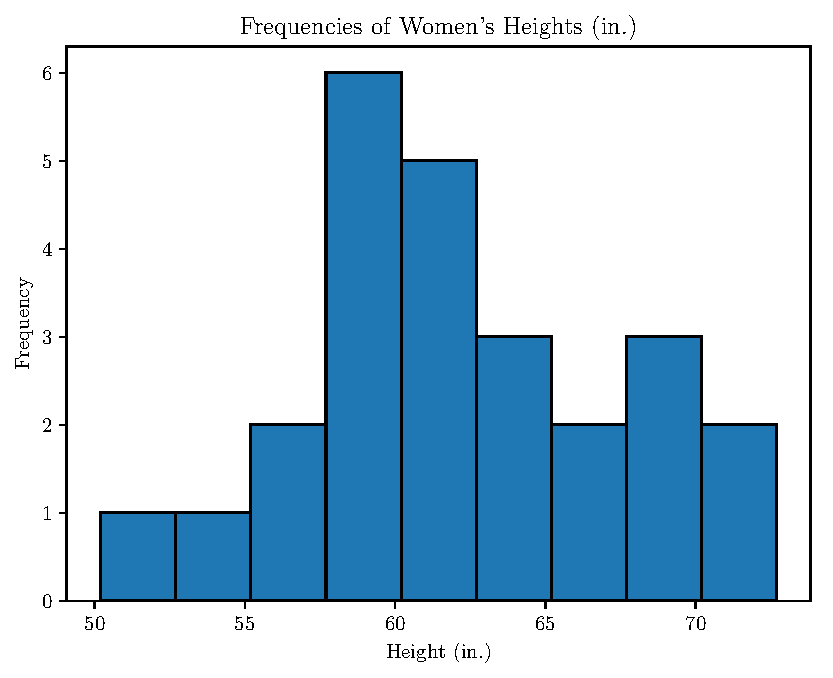
\includegraphics[width=0.85\textwidth]{plots/histogram.pdf}
        \end{figure}
      \item Pie chart:
        \begin{figure}[H]
          \centering
          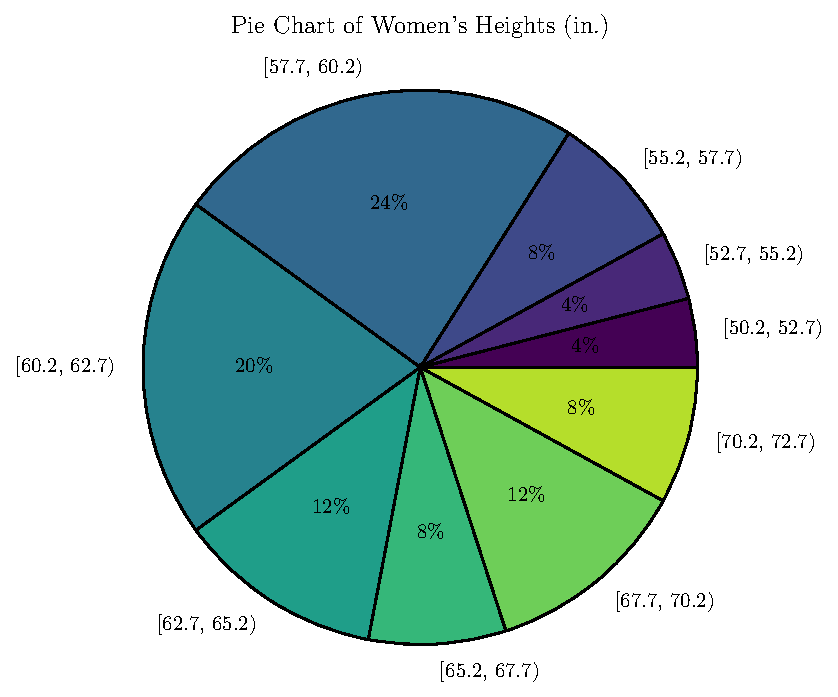
\includegraphics[width=0.85\textwidth]{plots/pie.pdf}
        \end{figure}
      \item Box plot:
        \begin{figure}[H]
          \centering
          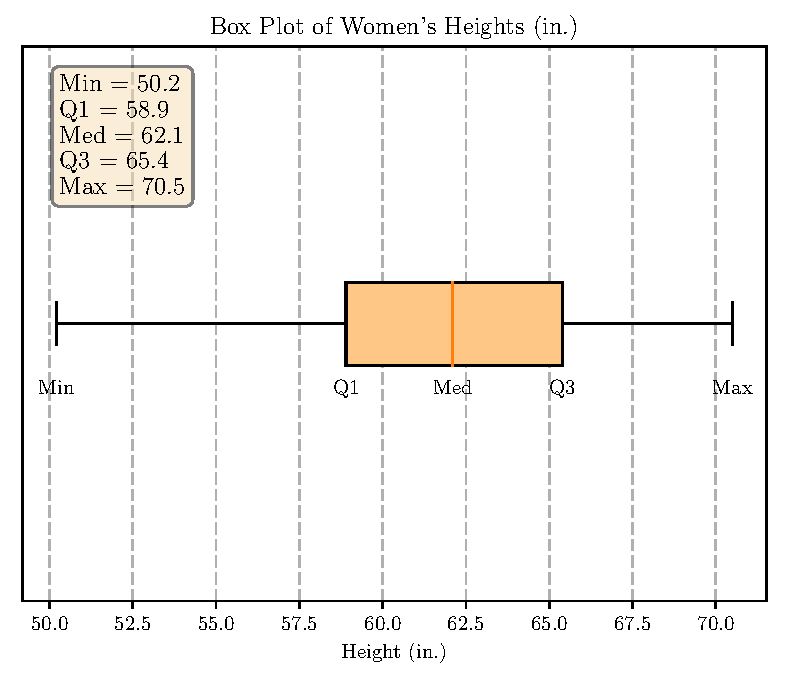
\includegraphics[width=\textwidth]{plots/box.pdf}
        \end{figure}
    \end{enumerate}

  % Question 2
  \item These data were used to compute the following sample summative statistics:
    \begin{table}[H]
      \centering
      \caption{Summative statistics about women's heights (in inches)}
      \begin{tabular}{l c}
  \hline
  Statistic & Value \\
  \hline
  Mean & 61.88 \\
  Median & 62.1 \\
  Midrange & 60.4 \\
  Mode & 68.5, 63.1, 62.4, 62.1, 59.3 \\
  Range & 20.3 \\
  Standard Deviation & 5.07 \\
  Variance & 25.68 \\
  \hline
\end{tabular}

    \end{table}

  % Question 3
  \item The data set possesses a left tail. This implies that is is not normally distributed; rather than being symmetric, it has a slight left skew.

  % Question 4
  \item In this scenario:
    \begin{enumerate}
      \item The mean increased. Let $\bar{x} = (\Sigma x)/n$ represent the original mean, where $x$ are the original data and $n$ is the original class size. Then $\bar{x}' = (100 + \Sigma x)/(n+1)$ is the new mean. Then we have:
        \begin{equation}
          \bar{x}' - \bar{x} = \frac{100n - \Sigma x}{n(n+1)}
        \end{equation}
      This difference is positive (indicating increase in mean) if $100 > (\Sigma x)/n = \bar{x}$; moreover, the mean of a data set cannot exceed its maximum value, so $\bar{x} \le 92$. Since $100 > 92$, the mean must have increased.
      \item For a sufficiently large class size, the median stays roughly the same. For very small classes (consider, say, a class of simply $\{71, 92\}$), the addition of a high score will appreciably change the median. However, for a class of large enough size for a ``normal distribution'' to be meaningful, this change is negligible. Loosely speaking, the new score, being greater than the original maximum, will shift the median up by half a value. Since the data are normally distributed, it is expected that the data are dense around the median, so this shift has very little impact. (It is even possible for this shift to have no impact if the median value is repeated.)
      \item The range increased. The original range was $92-71=21$. The new range is $100-71=29$, an obvious increase.
      \item The interquartile should stay roughly the same. Q1 and Q3 are both shifted slightly to the right by the new score, so their difference does not change by much, if at all. (A similar argument can be made that the interquartile range represents the ``middle 50\%'' of the data. Adding a single extreme value is unlikely to change this.)
      \item The standard deviation increases. Intuitively, the standard deviation expresses how ``spread out'' the data are, so adding an extreme value will increase it.
    \end{enumerate}

  % Question 5
  \item We examine the hypothesis:

    \textbf{Null:} Age and music preference are independent. \newline
    \textbf{Alternate:} Music preference is dependent on age.

  With the data:
    \begin{table}[H]
      \centering
      \caption{Music Preference by Age Group}
      \begin{tabular}{l | c c c c}
        \hline
        & \multicolumn{4}{c}{Age Group} \\
        & 15-24 & 25-34 & 35-44 & 45-54 \\
        \hline
        \multirow{2}{*}{Classical} & 12 & 37 & 72 & 85 \\
        & 10.7\% & 18.9\% & 40.4\% & 38.1\% \\
        \hdashline
        \multirow{2}{*}{Rock} & 89 & 106 & 64 & 100 \\
        & 79.5\% & 54.1\% & 36.0\% & 44.8\% \\
        \hdashline
        \multirow{2}{*}{Country} & 11 & 53 & 42 & 38 \\
        & 9.8\% & 27.0\% & 23.6\% & 17.0\% \\
        \hline
        \multirow{2}{*}{\textbf{Total}} & 112 & 196 & 178 & 223 \\
        & 100\% & 100\% & 100\% & 100\% \\
        \hline
      \end{tabular}
    \end{table}
  There are a few noticeable trends in the data; for instance, older participants were significantly more likely to prefer classical music than their younger peers, while younger participants were much more likely to enjoy rock music. As such, we conclude:

  Reject the null hypothesis. Support the alternate hypothesis. The data do support that music preference is dependent on age.

  \item For extra credit, the ``68-96-99.7 rule'' applies to normally distributed curves. 68\% of the data fit in between one standard deviation of the mean. 95\% of the data fit in between two standard deviations of the mean. 99.7\% of the data fit in between three standard deviations of the mean. This is called the empirical rule.
\end{enumerate}
\end{document}
